\chapter{Elastic modelling}
\label{chp:6}
\graphicspath{{chapter_6_Elasticmodelling/figures/chapter_6.tex}}% path to the figures folder of this chapter

%\section{Introduction}
This chapter discusses the different elastic modelling approaches and will present the results. The properties used in this analysis are based on the ABS blend specified in the the Ultimaker technical data sheet \cite{Ultimaker2018TechnicalABS}.

%\section{%Introduction}
%In this chapter the procedure and the results of the RVE homogenization model will be explained. The RVE homogenization model produced by Miguel Bessa \cite{bessa2017a} was originally developed to calculate the elastic properties of a random long fiber composite model. This was modified to be applied for FFF applications. The FFF mesostructure shows periodic porosity due to the process of sintering roads to eachother. Due to this periodicity a RVE could be defined, this was done in last chapter \ref{chp:4meso}. After the RVE has been meshed and an elongation is applied in a FEA, the internal stresses are saved and used in the homogenization method. The result is a compliance matrix for orthotropic materials that can be used to determine the elastic properties in the three principle directions, the theory behind this is discussed in the literature review \ref{chp:lit_rev}.
%These elastic properties can also be determined by conducting experimental tensile tests. To verify the model, multiple tensile tests were conducted in the three principle directions. These should show similar elastic properties as obtained in the RVE model. Since it was observed that the mesostructre of the analysed parts (as is shown in \ref{fig:ABS100yxmiddle}) is significantly different from the mesostructure observed in the literature, therefore the response of both the homogenization model and empirical test should also differ. If the mesostructure in chapter \ref{chp:4meso} is observed closely, one can conclude that the upper void is filled, in contrast to the mesostructure from the literature. This implies that the elastic properties in the 2 direction (xy) is larger than the results observed from the literature. 

\section{Methods and procedures}
\subsection{RVE homogenization model}
The RVE homogenization model is a combination of a Matlab (version 2018b) code of multiple scripts and functions where parameters for the RVE are assigned and where the results of the FEA are processed to obtain the elastic properties. The Matlab code designs an RVE based on the line width and thickness of the road structure as can be seen in figure \ref{fig:Roadstructure2}. Additionally, multiple RVE's can be stacked and the orientation of  layers can be altered according to the composite notation. The resulting RVE is presented in chapter 4. The design is exported to Abaqus (version 2018) , and is meshed with elements of a specific size. 
The finite element analysis includes an implicit model where the design is quasi-statically loaded with a 0.03 strain. Periodic boundary conditions are applied to the opposing faces of the RVE to simulate a larger solid, in figure \ref{fig:facesRVE} the RVE is defined with the different faces. When the properties of the 1 direction are determined, face 1 is loaded while face 3 is constrained. Periodic boundary conditions, simulating the stresses on the opposing faces, are applied. Face 6 is linked with 5, and face 4 is linked with 3. 
The internal stresses from the FEA in Abaqus are imported to Matlab and are used in the homogenization step according to equation \ref{eqn:homogenization}. After this step the compliance matrix can be calculated and the elastic properties can be extracted. These properties are saved for the specific settings used to generate the RVE design. 
A convergence study was conducted to determine the appropriate mesh size of the RVE. 
%To know what element size is appropriate for the mesh a convergence study was conducted. In this convergence study different sizes of elements are analyzed with the FEA model. The goal is to obtain a size large enough that gives a similar response to results with finer elements. 
%Similarly, a convergence study is conducted with the amount of pores in the RVE. Ideally (and according to the literature) one pore for a RVE is sufficient. However, to be sure that the response will not differ significantly (and therefore the definition of an RVE, which is the smallest volume element that is representative for the macrostructure) different amounts of pores are analyzed in the homogenization model to find the smallest RVE.

\begin{figure}[htb]
    \centering
    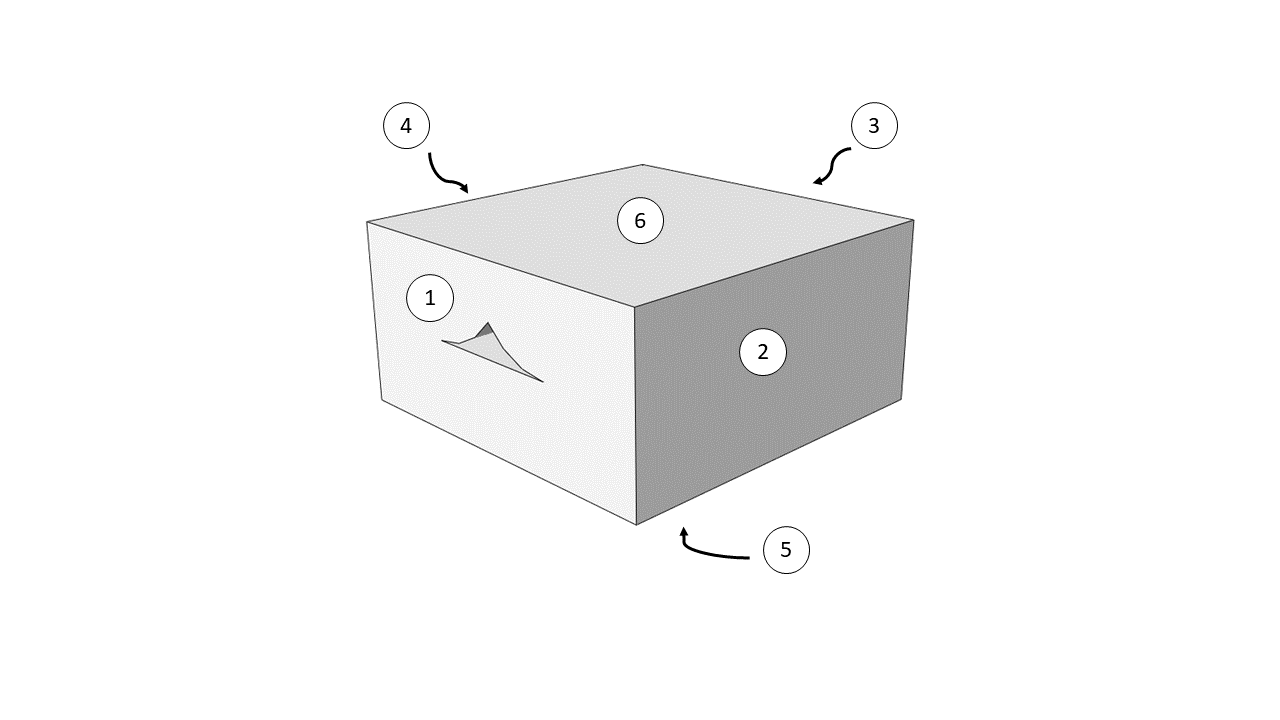
\includegraphics[width=0.80\textwidth]{chapter_6_Elasticmodelling/figures/facesRVE.png}
    \caption{RVE with the defined faces where the load and periodic boundary conditions are applied }
    \label{fig:facesRVE}
\end{figure}

\subsection{Mesh}
For this solid model a mesh of first order 3D hex-dominated elements was chosen and supplemented with wedge type triangular prisms. Hex-dominated elements are preferred for simple geometries since these are more accurate due to the degrees of freedom (8 nodes in 3 DOF). Additionally, tetrahedrons are prone to volumetric locking, generating an artificially stiff response. 
To apply periodic boundary conditions on the faces of the RVE, the seed of nodes should be identical on opposite faces. To achieve these requirements the RVE is divided in partitions as can be seen in figure \ref{fig:partition}.

%partitions here
\begin{figure}[htb]
    \centering
    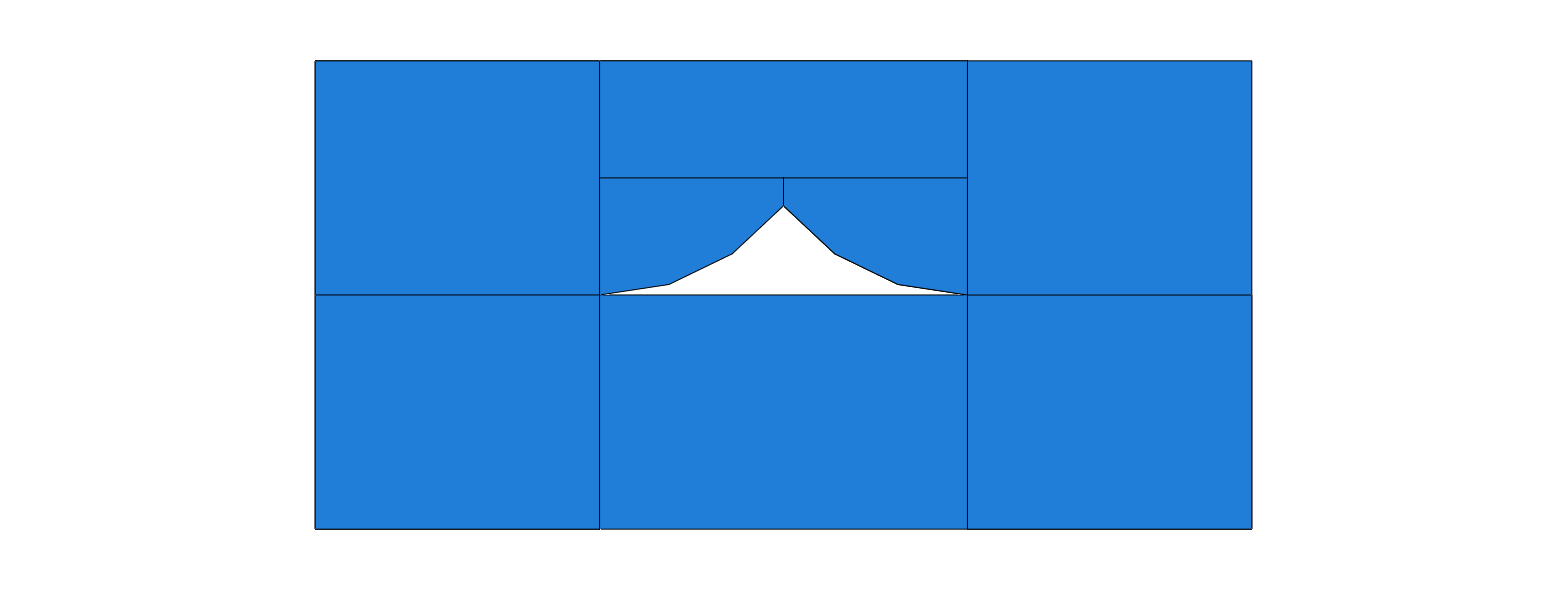
\includegraphics[width=0.60\textwidth]{chapter_6_Elasticmodelling/figures/partition.png}
    \caption{RVE with partitions to generate a evenly distributed hexahedral mesh}
    \label{fig:partition}
\end{figure}

The results from the homogenization model seemed to be insensitive for mesh size, as they did not alter significantly for an element size smaller than 0.05mm (1/8 of the RVE width, which is quite a coarse mesh ). The results also did not seem to alter with multiple RVEs used in the simulation. Since the homogenization simulations are not computationally intensive, a fine mesh with a global size of 0.01mm was chosen as is shown in figure \ref{fig:mesh}.

%Element Mesh here
\begin{figure}[htb]
    \centering
    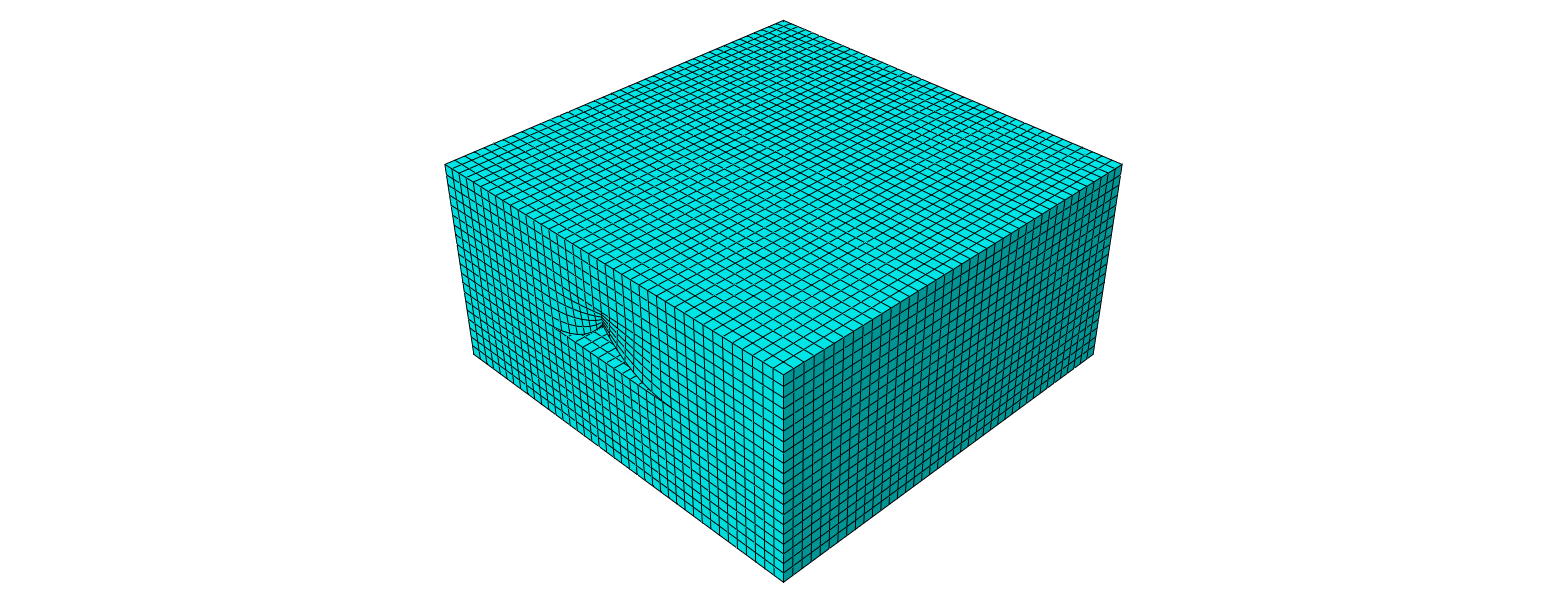
\includegraphics[width=0.90\textwidth]{chapter_6_Elasticmodelling/figures/mesh.png}
    \caption{The meshed RVE}
    \label{fig:mesh}
\end{figure}

\subsection{Voigt model}
Additionally to the RVE homogenization model, the analytical predictions by the Voigt model is also used to compare the elastic properties for different orientations. The Voigt model is explained in chapter 2 (equation \ref{eqn:Voigt}). The cavity in direction 2 and 3 is not constant and will therefore generate less accurate results. For this analysis, a cavity density is considered equal to the largest cavity surface in the corresponding direction. This will most likely under-predict the elastic properties due to decrease of the cavity along the cross section. Additionally, it should be noted that here also full healing (homogeneous bulk material) is considered, theoretically this should not influence the elastic properties, since the healing region that affect material properties is very thin and will likely only alter non-linear properties. 

\section{Results}
In figure \ref{fig:Elasticproperties} and table \ref{tab:Elasticproperties} the results are presented of for the FEA of the RVE and the analytical predictions as compared to the empirical data for the elastic properties.  The models are plotted as a function of the line ratio, which is the line height divided by the line width. Empirical measurements were only made for samples with a line width of 0.4 mm and a line height of 0.2mm.

\begin{figure}[htb]
    \centering
    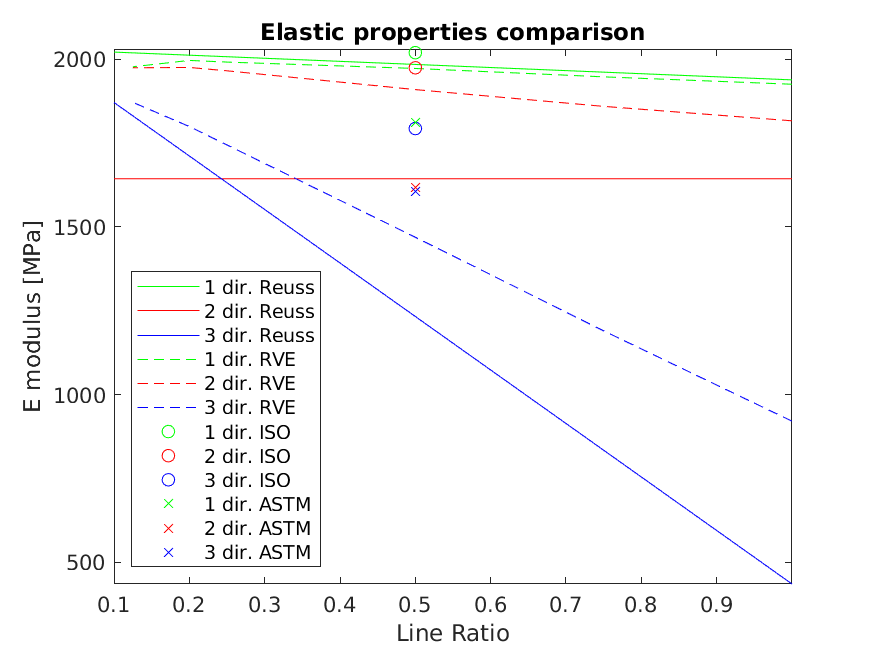
\includegraphics[width=0.80\textwidth]{chapter_6_Elasticmodelling/figures/Elasticproperties.png}
    \caption{Elastic properties for different aspect ratios ($l_h/l_w$ comparison between simulated RVE, experimental ISO 527 and ASTM D 3039 method, and according to the Voigt model.}
    \label{fig:Elasticproperties}
\end{figure}

\begin{table}
\caption{Elastic properties of different methods in the 3 principal directions}
\label{tab:Elasticproperties}
\begin{tabular}{p{2.2cm}p{2.2cm}p{2.2cm}p{2.2cm}p{2.2cm}}
 \hline
direction & $E$ Voigt [MPa] & $E$ RVE [MPa]& $E$ ISO [MPa]& $E$ ASTM [MPa] \\ 
\hline
1 (YX[0]) & 1984 & 1972 & 2019 & 1811 \\
2 (XY[0]) & 1643 & 1909 & 1974 & 1616 \\
3 (ZY[0]) & 1233 & 1469 & 1793 & 1563 \\
 \hline
\end{tabular}
\end{table}

\section{Discussion}
\subsubsection{Experimental elasticity}
The results in the previous section show the two approaches as a function of the aspect ratio including the results from experimental testing. In chapter 5 the effect of the sample shape on the properties is discussed. The ISO samples will probably over-estimate the elastic properties in the 2 and 3 direction due to extra wall layers that are implemented, this is in line with the observations of the models and the ASTM sample. The results from the ASTM sample should in theory give the most representative elastic response. However, since the large surface roughness and non-constant sample cross section, it can be difficult to exactly measure the cross sectional area. Additionally, since there is no perfect healing, there may be some localized damage (e.g. debonding) which would lead to a decrease in the $E$ modulus. Surprisingly, the 1 and 2 empirically tested directions significantly under-perform compared with the results from the models. This might be due to inaccuracies in the measurements. Since the surface is very rough, the measured surface might be larger than the actual surface, generating low elasticity for the empirical results. Interestingly, the 3 direction in both empirical methods show a better performance compared with the models. This can probably be explained due to the large cavity area that is assumed in the 3 direction. This area would in reality be smaller, and would have blunted corners.

\subsubsection{Voigt model}
The Voigt model makes some drastic simplifications in the 2 and 3 direction as is described in "Methods and procedures" of this chapter. Since the largest cavity fraction is assumed, the model will significantly under-predict the elastic properties. 

\subsubsection{RVE model}
The FEA of the RVE still leads to a lower result compared with both the empirical tests. The RVE model is in general closest to the empirical results, for the 1 and 2 direction it is slightly lower than the ISO test, and higher than the ASTM test. For the three direction, it is lower than both tests for reasons mentioned before.

\section{Conclusion}
The models and empirical tests show subtle differences with respect to the each other. In general the ISO samples have the highest results due to the included wall layers. The Voigt and RVE model show similarities, but the RVE model has less problems with simplifications and shows more consistency with the empirical results. The ASTM samples show some complications  in the 2 directions due to the large surface roughness in the 2 direction, which seems to have approximated the response obtained for the 2 and 3 directions.
The varying empirical results display the demand for a good standard that produce consistent representative results. To correctly compare the models with the empirical tests, and the dependency on the line ratio, more experimental data should be gathered for different line ratios and a good measuring standard should be created for FFF products.
Research question 4 in Chapter \ref{chp:hypothesis} can partly be answered on the elastic properties of of FFF products. The elastic properties differ significantly in the 2 and 3, especially for larger aspect ratios. There is still little relevant experimental data available to make a strong statement on the predictive power of the different models. These do however, indicate the stiffest directions accurately. 
%---------------------------------------------------------------------------------------------------------------------------

